\documentclass[landscape]{sciposter}

\usepackage{a0size}
\usepackage{amsmath}
\usepackage{amssymb}
\usepackage{multicol}
\usepackage[english]{babel}
\usepackage{setspace}
\usepackage[pdftex,final]{graphicx} 
\usepackage{epsfig}
\usepackage{dsfont}
\usepackage{bm}
\usepackage{color}
\usepackage{url}


\newcommand{\refeqn}[1]{ (\!\!~\ref{eq:#1}) } % gives references to
\newcommand{\refthm}[1]{ (\!\!~\ref{#1}) }    % equations or theorems





\definecolor{BoxCol}{RGB}{0,120,0 }


\definecolor{SectionCol}{rgb}{1,1,1}
% uncomment for dark blue \section text
\definecolor{TextColG}{rgb}{0,0.5,0}
\definecolor{TextColR}{rgb}{0.5,0,0}
\newcommand{\Rcolor}{\textcolor{TextColR}}
\newcommand{\Gcolor}{\textcolor{TextColG}}

\definecolor{OSUGreen}{RGB}{0,120,0}
\newcommand{\Green}{\textcolor{OSUGreen}}

\definecolor{Gold}{RGB}{255,215,0}
\newcommand{\Gold}{\textcolor{Gold}}

\definecolor{RoyalPurple}{RGB}{120,81,169}
\newcommand{\Purple}{\textcolor{RoyalPurple}}

\definecolor{Black}{RGB}{0,0,0}
\newcommand{\Black}{\textcolor{Black}}


%%%%%%%%%%%%%%%%%%%%%%%%%%%%%%%%%%%%%%%%%%%%%%%%%%%%%%%%%%%%%%%%%%
%My new commands







%%%%%%%%%%%%%%%%%%%%%%%%%%%%%%%%%%%%%%%%%%%%%%%%%%%%%%%%%%%%%%%%%%

%-------------------------------------------------------------------------------------------------------
\title{P vs NP}




\author{ \hspace{0 in} Chaskin Saroff, Alexander Jansing }

\institute{\Black{ \hspace{0 in} State University of New York at Oswego\\ \hspace{0 in} Department of Mathematics\hspace{3.1 in}
\\Oswego, NY, USA\\}}

\email{csaroff@oswego.edu}, \email{ajansing@oswego.edu}

% The following commands can be used to alter the default logo settings
\leftlogo[2]{oswegologo}  % defines logo to left of title (with scale factor)
\rightlogo[1.0]{oswegologo}  % same but on right

%-------------------------------------------------------------------------------------------------------
\begin{document}

%define conference poster is presented at (appears as footer)
\conference{Spring 2015 - Number Theory}

\maketitle

% 
\begin{abstract}
\begin{center}
\parbox{35 in}{\Large The abstract should be a brief overview of the project.  Keep specialized notation to a minimum; try to explain to a general audience what the project is about in a way to draw a viewer's attention.  Some say that the abstract of a poster should have a larger font size, to catch a viewer's eye as he/she passes along but if you don't want to have a larger font size then delete the sizing command at the start of this textbox. You can also make your abstract horizontally skinnier by decreasing the number in the parbox qualifier.}
\end{center}
\end{abstract}

%%% Begin of Multicols-Enviroment -- 
\begin{multicols}{4}

%-------------------------------------------------------------------------------------------------------
\section*{INTRODUCTION}
% To leave a section number out, put a star in.

Algorithmic time complexity has interesting applications to Number Theory and much more.  How long does it take to sort a list of a million numbers?  
\\
\\
Can  large primes be factored quickly?  If the solution to a problem can be verified in polynomial time, can it be solved in polynomial time?  \cite{CD}.
\\
\\
If P=NP, then cryptographic security systems, as they stand now, are broken.  It is as easy to decode encrypted messages as it to encode them.
\\
\\
Solving this problem is interesting and valuable because of its implications to data security as well as speeding up computers.
%-------------------------------------------------------------------------------------------------------
\section{HISTORY}
The P vs NP question is famous for being one of the most accessible millennium prize questions\cite{Sipser}. It began in 1936 when Alan Turning developed a theoretical computational model, which later became a useful theoretical model for computation. Although, the original model soon failed as the needs for time and memory were not accounted for\cite{Fortnow}.
\\
Throughout the 1960's, 70's, and 80's the understanding of time complexity developed rapidly. Several mathematicians and computer scientists proved many problems could be solves in polynomial time and created notations that illustrated the time (and sometimes, space) complexity of their calculations. In the 1970's \textbf{NP}-completeness became one of the most insightful and fundamental theories in mathematics and furthered out knowledge of the combinatorial difficulties of many problems that seem to lack solutions that can be found in polynomial time\cite{Fortnow}.

%-------------------------------------------------------------------------------------------------------
\section{NOTATION}

Some good rules for mathematical notation:
\\
\\
\begin{itemize}
\item P = Set of all problems which are solvable in polynomial time.
\item NP = Set of all problems whose solutions can be verified in polynomial time.
\item NP-Hard = Set of all problems that are at least as hard as the problems in NP.
\item NP-Complete = Set of all problems that are in both NP and NP-Hard.
\end{itemize}

\

\begin{center}

\includegraphics[scale = 2.6]{oswegologo}
\end{center}

%%-------------------------------------------------------------------------------------------------------

\section{FIGURES}
Blanks are bad for business. Fill your space with figures, if you have nothing else.


\begin{center}

\includegraphics[scale=.8]{Time_Complexity_Line.png}
\end{center}

\begin{figure}
\centering

\includegraphics[scale=0.30]{P_vs_NP_Euler_Diagram}
\caption{Euler Diagram showing P vs NP vs NP-Hard}
\end{figure}
\\
\begin{figure}
\centering
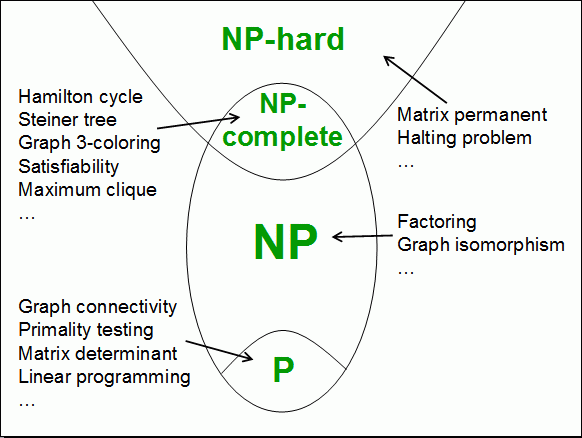
\includegraphics[scale=1.0]{examples_time_complexity.png}
\caption{P, NP, NP-Hard Problems}
\end{figure}

Don't forget that you may need to scale your images so that they fit in the columns.  An oversized image will wreak havoc on the appearance of your poster.

%%-------------------------------------------------------------------------------------------------------

\section{The Multicols Environment}

The \{4\} after the multicols command tells the compiler to divide the width of the poster into four equal columns, and adjust the length of the poster as necessary.  If you have less content or wide figures then you might be better off with fewer columns -- three is fine, but 2 starts to make things look sparse.
\\
\\
The thing is, you need to have enough material to fill up the poster and prevent a giant white spot at the bottom.  That's just awful-looking!


%-------------------------------------------------------------------------------------------------------
\section{MORE SECTIONS!}

The more we know about our degradation function H and our noise function $N$, the better our estimate of $f(x,y)$ will be. In the spatial domain, we represent our degraded function as: 
\\
\begin{equation}
g(x,y)=h(x,y) \ast f(x,y) + \eta(x,y)
\label{eq:conv}
\end{equation}
\\
where $h(x,y)$ is the spatial representation of the degradation function. 

%-------------------------------------------------------------------------------------------------------
\section{References with BibTeX}

Open the references.bib file and check out the sample citation entries.  If you require different kinds of entries, search ``Bibtex entries'' on the internet and a whole array of options will be available.  Each entry has a name that you'll use in the tex file when you're typing to call up that citation.
\\
\\
Once your references are each formatted as a BibTeX entry, you can cite them using the cite\{\} command.  in the tex tile.  There are several examples here in this document.  If you don't actually have a citation in the text for something, you can use the command ``nocite'' in front of the bibliography style command in your file.  
\\
\\
You need to cite data sources and any specialized software that you've used (GAP, Sage, R).  Usually specialized software programs have information on their webpages about how to properly cite the software.  
\\
\\
Now you need to compile your tex file.  First, make sure references.bib and your tex file are in the same folder.  Then latex compile your tex source file.  If you're using TeXShop or TeXWorks, then the next step is to Bibtex compile your tex source file.  Then latex compile your tex source file TWICE more.  It's crazy!  If you're using other software, sometimes you just need to latex compile your tex source file 3-4 times.  When in doubt, the internet can help you fgure out the procedure.

\begin{figure}
\centering

\includegraphics[scale = 2.0]{oswegologo}
\end{figure}



%---------------------------------------------------------------------------------------------------------------
\section{ACKNOWLEDGEMENTS}

Professor Elizabeth Wilcox, for her review and guidance throughout the research and development of this project

%-------------------------------------------------------------------------------------------------------

\nocite{WinNT}
\nocite{GAP4}
\bibliographystyle{plain}
\bibliography{references}

\end{multicols}

% This makes a green bar along the bottom of the poster content.  If you want to add a message, feel free.
\section*{ }

\end{document}
